\begin{figure}
	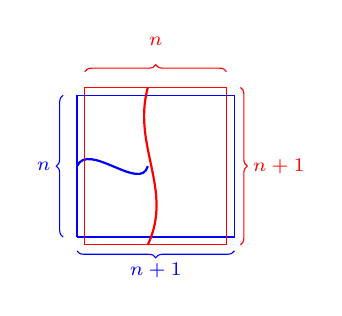
\begin{tikzpicture}[scale = 0.20]
		\draw[blue] (0, 0) -- (10, 0) -- (10, 9) -- (0, 9) -- (0, 0);
		\draw[blue, decoration = {brace, mirror, raise = 5pt}, decorate] (0, 0) -- node[below = 6pt] {{\scriptsize $n + 1$ }} (10, 0);
		\draw[blue, decoration = {brace, raise = 5pt}, decorate] (0, 0) -- node[left = 6pt] {{\scriptsize $n$ }} (0, 9);
		\draw[blue, thick] (0, 4.5) to[out = 65, in = -105] (4.5, 4.5);
		
		\draw[red] (0.5, -0.5) -- (9.5, -0.5) -- (9.5, 9.5) -- (0.5, 9.5) -- (0.5, -0.5);
		\draw[red, decoration = {brace}, decorate] (0.5, 10.5) -- node[above = 6pt] {{\scriptsize $n$ }} (9.5, 10.5);
		\draw[red, decoration = {brace, mirror, raise = 5pt}, decorate] (9.5, -0.5) -- node[right = 6pt] {{\scriptsize $n+1$ }} (9.5, 9.5);
		\draw[red, thick] (4.5, -0.5) to[out = 65, in = -105] (4.5, 9.5);
	\end{tikzpicture}
	\vspace{-12pt}
	\caption{Esboço dos eventos $\HC(n+1, n)^c$ e $\VC(n, n+1)$.} 
	\label{fig-caixas-sobrepostas}
\end{figure}